\documentclass[11pt,a4paper]{article}

\usepackage[utf8]{inputenc}		% Configuro la codificación
\input{.command.tex}
% En el siguiente archivo se configuran las variables del trabajo práctico
%% \providecommand es similar a \newcommnad, salvo que el primero ante un 
%% conflicto en la compilación, es ignorado.

% Al comienzo de un TP se debe modificar los argumentos de los comandos


\providecommand{\myTitle}{TRABAJO PRÁCTICO Nº0}
\providecommand{\mySubtitle}{Promedio móvil de módulos de complejos}

\providecommand{\mySubject}{Algoritmos y Programación II (95.12)}
\providecommand{\myKeywords}{UBA, Ingeniería, C++, 95.12, Algoritmos y Programación}

% No es necesario modificar este
\providecommand{\myHeaderLogo}{header_fiuba}

\providecommand{\myAuthorSurname}{Andreasen & Manso}
\providecommand{\myTimePeriod}{Año 2016 - 2\textsuperscript{do} Cuatrimestre}


% Crear los integrantes del TP con el comando \PutMember donde
%%		1) Apellido, Nombre
%%		2) Número de Padrón
%%		3) E-Mail (Si el mail contiene '_', escribirlos como '\_'
\providecommand{\CoverMembers}[0]
{		\PutMember{Andreasen, Ricardo} {96322} {ra\_95\_1@hotmail.com} 
		\PutMember{Manso, Juan} {96133} {juanmanso@gmail.com}
}

\providecommand{\myLstLanguage}{C++}

\Pagebreakfalse		% Setea si hay un salto de página en la carátula
\Indexfalse
\Siunixfalse		% Si quiero utilizar el paquete, \siunixtrue. Si no \siunixfalse
\Listingstrue		% Idem con paquete listings (programación)
\Keywordsfalse
				% Archivo con los comandos globales como Título y autores
%Preambulo para articulo científico de LaTeX

\usepackage[a4paper,left=3cm,right=3cm,bottom=3.5cm,top=3.5cm]{geometry} 	% Configuro la geometría del papel
%\usepackage{microtype}														% Mejora el "spacing" de las palabras
\usepackage[spanish]{babel} 												% Compatibilizo los signos del español
	\addto\captionsspanish{\renewcommand{\tablename}{Tabla}}				%% Redefino nombres preestablecidos por Babel
	\addto\captionsspanish{\renewcommand{\listtablename}{Índice de tablas}}	%% y así en vez de Cuadro dirá Tabla.
\usepackage{amsmath, amsfonts, amssymb}										% Entornos matemáticos, fuentes y símbolos
\usepackage{graphicx}														% Necesario para insertar figuras
\usepackage{fancyhdr}														% Para manipular headers y footers
\usepackage[usenames]{color}											% \color{color deseado} {lo que querés que tenga color}
\usepackage{subcaption}														% Permite captions del tipo 1a, 1b
\usepackage{multirow}														% Para tablas
\usepackage{float}

\ifListings
	\usepackage{listingsutf8}

	\definecolor{mygreen}{rgb}{0,0.6,0}
	\definecolor{mygray}{rgb}{0.5,0.5,0.5}
	\definecolor{mymauve}{rgb}{0.58,0,0.82}
	
	\providecommand{\lstinputpath}[1]{\lstset{inputpath=#1}}

	\lstset{
		backgroundcolor=\color{white},   % choose the background color; you must add \usepackage{color} or \usepackage{xcolor}
		inputencoding=utf8/latin1,
		basicstyle=\ttfamily\footnotesize,        % the size of the fonts that are used for the code
		breakatwhitespace=false,         % sets if automatic breaks should only happen at whitespace
		breaklines=true,                 %% sets automatic line breaking
		captionpos=t,                    %% sets the caption-position to top 
		commentstyle=\color{mygreen},    % comment style
		deletekeywords={...},            % if you want to delete keywords from the given language
		escapeinside={\%*}{*)},          % if you want to add LaTeX within your code
		extendedchars=true,              % lets you use non-ASCII characters; for 8-bits encodings only, does not work with UTF-8
		frame=single,	                 %% adds a frame around the code
		keepspaces=true,                 % keeps spaces in text, useful for keeping indentation of code (possibly needs columns=flexible)
		keywordstyle=\color{blue},       % keyword style
		language=C++,		 	 %% the language of the code
		otherkeywords={*,...},           % if you want to add more keywords to the set
		numbers=left,                    %% where to put the line-numbers; possible values are (none, left, right)
		numbersep=5pt,                   %% how far the line-numbers are from the code
		numberstyle=\tiny\color{mygray}, % the style that is used for the line-numbers
		rulecolor=\color{black},         % if not set, the frame-color may be changed on line-breaks within not-black text (e.g. comments (green here))
		showspaces=false,                % show spaces everywhere adding particular underscores; it overrides 'showstringspaces'
		showstringspaces=false,          % underline spaces within strings only
		showtabs=false,                  % show tabs within strings adding particular underscores
		stepnumber=1,                    % the step between two line-numbers. If it's 1, each line will be numbered
		stringstyle=\color{mymauve},     % string literal style
		tabsize=4,	                   % sets default tabsize to 2 space
		title={\protect\filename@parse{\lstname}\protect\filename@base\text{.}\protect\filename@ext}	 %% show the filename of files included with \lstinputlisting; also try caption instead of title
	}
	 \usepackage{algpseudocode}						% Para pseudocodigo
	 \renewcommand{\algorithmicwhile}{\textbf{mientras}} 
	 \renewcommand{\algorithmicdo}{\textbf{hacer}} 
	 \renewcommand{\algorithmicfor}{\textbf{para}}
	 \renewcommand{\algorithmicreturn}{\textbf{devolver}}
	 \renewcommand{\algorithmicend}{\textbf{fin}} 
	 
	 \newcommand{\rpm}{\raisebox{.2ex}{$\scriptstyle\pm$}}  
\fi

\ifSiunix
\usepackage{siunitx}											% Unidades: \SI {cantidad} {\unidad} (necesita texlive-science)
	\sisetup{load-configurations = abbreviations}							% Habilita poner \cm en vez de \centi\metre
	\sisetup{output-decimal-marker = {,}}									% Cambia los puntos decimales por comas
\fi

\usepackage{booktabs}														% Permite hacer tablas sin separadores en el medio
\usepackage{placeins}														
		\let\Oldsection\section												%% Permite que los flotantes (como figuras) no aparescan
	\renewcommand{\section}{\FloatBarrier\Oldsection}						%% antes o después de su sección correspondiente.
		\let\Oldsubsection\subsection
	\renewcommand{\subsection}{\FloatBarrier\Oldsubsection}		
		\let\Oldsubsubsection\subsubsection
	\renewcommand{\subsubsection}{\FloatBarrier\Oldsubsubsection}
\usepackage{hyperref}														% Debe ser agregado al final del preambulo

\hypersetup
{    bookmarks=true,         % show bookmarks bar?
     unicode=false,          % non-Latin characters in Acrobat’s bookmarks
     pdftoolbar=true,        % show Acrobat’s toolbar?
     pdfmenubar=true,        % show Acrobat’s menu?
     pdffitwindow=false,     % window fit to page when opened
     pdftitle={\myTitle},    		 % title
     pdfauthor={\myAuthorSurname},   % author
	 pdfcreator={\myAuthorSurname},	 % creator = author
     pdfsubject={\mySubject},		 % subject of the document
     pdfkeywords={\myKeywords},
     colorlinks=true,        % false: boxed links; true: colored links
     linkcolor=black,        % color of internal links (change box color with linkbordercolor)
     citecolor=black,        % color of links to bibliography
     filecolor=magenta,      % color of file links
     urlcolor=cyan           % color of external links
}

%Configuro la pagina con los encabezaos y pies de paginas
\pagestyle{fancy}										% Para agregar encabezados y pie de paginas	
\lhead{\mySubject}										% Encabezado izquierdo
\rhead{\includegraphics[scale=0.15]{\myHeaderLogo}} 	% Encabezado derecho (logo de la FIUBA)					


% Defino el path de los includegraphics
\graphicspath{{./Figuras/}}		% Directorio que contiene los graficos

% Defino el path para los input de .tex y de .eps
\makeatletter
\def\input@path{{./Figuras/}{./Secciones/}{./Cover_page/}}
\makeatother

% Defino el path del listings
\lstinputpath{../Programa/test}


\begin{document}
		% Carátula (formal o simple,_formal o _simple respectivamente),
		% Resumen e Índice (si es necesario configurar en config.tex) del informe
		\begin{titlepage}
	
		\thispagestyle{empty}

		\begin{center}
			
\includegraphics[scale=0.3]{fiuba}\\
			\large{\textsc{Universidad de Buenos Aires}}\\
			\large{\textsc{Facultad De Ingeniería}}\\
			\small{\myTimePeriod}
		\end{center}

		\vfill

		\begin{center}
			\Large{\underline{\textsc{\mySubject}}}
		\end{center}

		\vfill

		\begin{tabbing}
			\hspace{2cm}\=\+\myTitle\\
				TEMA: \mySubtitle\\
				FECHA: \today\\
			\\
			\MembersHeader
			\CoverMembers
		\end{tabbing}

		\begin{abstract}
			% Ejemplo de Resumens
%% MANTENER EL NOMBRE %%
	El siguiente trabajo práctico tiene como objetivo el diseño e implementación de un programa en C++, ejercitando los conceptos básicos del lenguaje y documentando dicha implementación.



		\end{abstract}

	\ifKeywords
		\begin{center}
			\emph{Palabras Clave: \myKeywords}
		\end{center}
	\fi	

		\vfill
	
\end{titlepage}

\ifPagebreak
	\thispagestyle{empty}
	\ifIndex
		\tableofcontents
%		\listoffigures
%		\listoftables
	\fi

	\pagebreak
\fi



	\setcounter{page}{1}
	\section{Diseño e implementación}	\label{sec:design}
		\subsection{Diseño del algoritmo}

En el presente informe se detalla la implementación de una herramienta para procesar señales moduladas en amplitud, de acuerdo al siguiente esquema:

\begin{figure}[h]
\centering
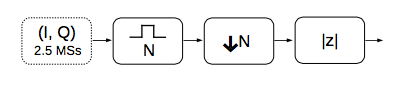
\includegraphics[width = 0.6 \textwidth]{flujo_senales}
\caption{Flujo de procesamiento de señales.}
\label{fig:flujo_senales}
\end{figure}

Se provee como entrada una secuencia de números complejos $(I[n],Q[n])$ que representan las muestras en fase y cuadratura de la señal modulada. Esta secuencia se pasa por un \textit{moving average}, un decimador y finalmente se le calcula el módulo punto a punto para obtener a la salida una secuencia de números reales $R[n']$.

En primer lugar se definió el algoritmo mediante el cual se realizaría el procesamiento de señales. 

Se tuvo en cuenta el hecho de que, a partir del \textit{downsampling}, se desecha una cantidad importante de muestras. Específicamente, si se fijó un parámetro de decimación $N$, de cada $N$ muestras procesadas sólo una es finalmente utilizada. Por lo tanto sólo hace falta realizar los cálculos para las muestras que sabemos van a ``sobrevivir'' la decimación.

Para cada muestra $n$, el \textit{moving average} realiza un promedio de las $N$ últimas muestras recibidas, es decir sigue la ecuación:

	\begin{equation*}
		 y[n] = \frac1N \sum_{k = 0}^{N-1} x[n-k]. 
	\end{equation*}

De lo anterior se sigue que cada muestra a la salida $y[n_0]$ es sólo función de los $N$ últimos valores a la entrada $x[n_0], x[n_0 - 1], \dots,  x[n_0 - N + 1]$. Los demás bloques de procesamiento sólo dependen del valor actual de su entrada, por lo que finalmente en el programa sólo hace falta recordar las últimas $N$ muestras que se recibieron para realizar los cálculos. 

Con estas observaciones en mente, se optó por el siguiente algoritmo de implementación:

	\begin{algorithmic}[H] % algorithmic fue el que pude hacer andar, porque me dejaba 
		       % redefinir las keywords. algorithm2e era mas lindo pero seteandolo
                       % con spanish y onelanguage mezclaba español con italiano.
		       % Si encontras uno que se vea mejor y en español es bienvenido.

		%\caption{Algoritmo para el procesamiento de las muestras.}
	
		\While{el \textit{stream} de datos no termine}
			\State $promedio := 0$
			\For{las N siguientes muestras}
				\State $promedio \gets promedio + x[n]$
			\EndFor
			\State $promedio \gets promedio / N$
			\Return $\sqrt{\mathbf{Re}\{promedio\}^2 + \mathbf{Im}\{promedio\}^2}$ 
		\EndWhile
	\end{algorithmic}

\newpage

\subsection{Implementación}
 De acuerdo a lo requerido, la implementación de la herramienta se realizó en C++, para entradas y salidas de texto en los formatos especificados. Para ello se aprovecharon las clases \texttt{cmdline} y \texttt{complex} provistas en el curso, para el manejo de argumentos y números complejos respectivamente.

 Con respecto al manejo de argumentos, para utilizar la clase \texttt{cmdline} hace falta definir la tabla de opciones que se esperan recibir, de tipo \texttt{option\_t}. Se optó por definirla dentro del \texttt{main} del programa, con las siguientes opciones:

%	\lstinputlisting[firstline=48, lastline=54]{main.cc}

\lstset{language=C++}
\begin{lstlisting}[frame=single]
static option_t options[] = {
	{1, "i", "input", "-", opt_input, OPT_DEFAULT},
	{1, "o", "output", "-", opt_output, OPT_DEFAULT},
	{1, "N", "n_decimator","500",opt_n_decimator, OPT_DEFAULT},
	{0, "h", "help", NULL, opt_help, OPT_DEFAULT},
	{0, },
};
\end{lstlisting}

Como es requerido, se definió a la cadena ``-'' (tercera columna de la tabla de opciones) como el valor por defecto para las opciones de entrada y de salida. De esta manera, ya sea que se haya omitido esa opción o se la especifique explicítamente para que asuma su valor por defecto, en ambos casos se  obtendrá el mismo resultado.

Además la clase \texttt{cmdline} pide especificar las funciones que se utilizarán para \emph{parsear} cada opción (5ta columna de la tabla) - se las definió en el mismo \texttt{main}. Para las funciones que parsean las opciones de entrada, salida y ayuda se aprovecharon las que ya estaban implementadas en el archivo \texttt{main.cc} provisto con la implementación de la clase \texttt{cmdline} del curso. Quedó por definir, entonces, el \texttt{parser} para el parámetro $N$ de decimación:


\lstset{language=C++} 
\begin{lstlisting}[frame=single]
static void
opt_n_decimator(string const &arg)
{
	istringstream iss(arg);

	// Intentamos extraer el N de la linea de comandos.
	// Para detectar argumentos que unicamente consistan de
	// numeros enteros, vamos a verificar que EOF llegue justo
	// despues de la lectura exitosa del escalar
	
	if(!(iss >> n_decimator) || !iss.eof()) {
		cerr << "non-integer factor: "
		     << arg
		     << "."
		     << endl;
		exit(1);
	}

	if (iss.bad()) {
		cerr << "cannot read integer factor."
		     << endl;
		exit(1);
	}
}
\end{lstlisting}

Como el método \texttt{parse} de \texttt{cmdline} ya le pasa al \texttt{parser} su valor por defecto si fue omitido, siempre esta función recibirá un argumento para $N$ (no necesariamente válido). Se intenta leer el mismo como un entero, y de fallar se anuncia el error y se termina el programa. 

Los argumentos se leen mediante \texttt{cmdline.parse($\cdot$)} a cada una de las variables estáticas definidas fuera del \texttt{main}:

 
\lstset{language=C++}
\begin{lstlisting}[frame=single]
static size_t n_decimator;	// Decimator Factor (factor positivo de decimacion)
static istream *iss = 0;	// Input Stream (clase para manejo de los flujos de entrada)
static ostream *oss = 0;	// Output Stream (clase para manejo de los flujos de salida)
static fstream ifs; 		// Input File Stream (derivada de la clase ifstream que deriva de istream para el manejo de archivos)
static fstream ofs;		// Output File Stream (derivada de la clase ofstream que deriva de ostream para el manejo de archivos)
\end{lstlisting}

Estas son las variables que se le pasan a \texttt{am\_proc} que es la encargada de implementar el algoritmo de la sección anterior, de manera que el \texttt{main} queda:


\lstset{language=C++}
\begin{lstlisting}[frame=single]
int
main(int argc, char * const argv[])
{
	cmdline cmdl(options);	// Objeto con parametro tipo option_t (struct) declarado globalmente.
	cmdl.parse(argc, argv);	// Metodo de parseo de la clase cmdline
	am_proc(iss, oss, n_decimator);	// Procesamiento AM
}
\end{lstlisting}

La función \texttt{am\_proc} está declarada en ``\texttt{am\_proc.h}'' y definida en ``\texttt{am\_proc.cc}''. Fuera de comprobar si hubo errores de lectura, su implementación es en escencia el pseudo-código de la sección anterior:

\lstset{language=C++}
\begin{lstlisting}[frame=single]
void am_proc(istream *is, ostream *os, const size_t& n_decimator){
	
	bool eof_flag=false;
	size_t i;
	complejo c, aux; // c tendra la suma y aux sera el que recibe el complejo del stream	


	// Si entra un archivo vacio (primero lee EOF), corta el for y luego el while, devolviendo un vacio

	while(!eof_flag){
		
		// Se suman los primeros 'n_decimator' numeros hasta que corte 
		for(i=1; i<=n_decimator && ((*is)>>aux); i++)
			c += aux;
	
		// Compruebo si se llego a EOF
		if(is->eof())
			eof_flag=true;

		if(is->bad()){ 
		// El for termino por no poder guardar el caracter en x
			cerr	<< "Error: Cannot read complex on input stream"
				<< endl;
			exit(1);
		}		

		// Realizo el proemdio movil
		c=c / n_decimator;
			
		// Imprimo el valor absoluto
		*os << c.abs()<<endl;
	}
	
	if(os->bad()){
		cerr	<< "Error: Cannot write output file"
			<< endl;
		exit(1);
	}

}
\end{lstlisting}



	\section{Proceso de compilación} 	\label{sec:comp}
		
Para el manejo del proyecto se optó por utilizar la herramienta \texttt{make} por sobre la compilación manual, dado que \texttt{make}, utilizando el archivo \texttt{Makefile}, evalua si los archivos fuente fueron modificados después de la compilación y sólo ejecuta los scripts necesarios. Además mantiene al proyecto ordenado y facilita su desarrollo. A continuación se presenta dicho archivo \texttt{Makefile} que se encuentra en el directorio que contiene todos los archivos fuente y se ejecuta desde la terminal de UNIX simplemente insertando el comando \texttt{make} o en su defecto \texttt{make all}. 

\lstinputlisting[language=make]{Makefile}



	\section{Corridas de prueba}
		
A continuación se presentan las corridas de prueba realizadas a lo largo del desarrollo. \\

\begin{figure}[H]
	\centering
		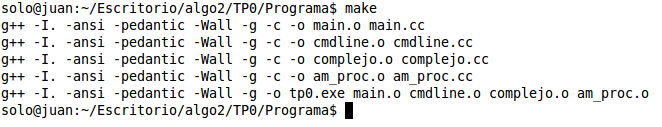
\includegraphics[width=1\textwidth]{compilacion.png}
	\caption{Compilación del programa.}
	\label{fig:corrida_makefile}
\end{figure}

En primera instancia se ve en la Figura \ref{fig:corrida_makefile} que la compilación del programa resulta satisfactoria según lo desarrollado en la sección \ref{sec:comp}.

Luego se probaron los ejemplos propuestos por las especificaciones:

\begin{figure}[H]
	\centering
		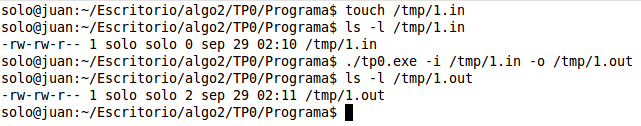
\includegraphics[width=1\textwidth]{prueba-1_con_problemas.png}
	\caption{Ejemplo 1 del enunciado del TP.}
	\label{fig:prueba1_con_prob}
\end{figure}


\begin{figure}[H]
	\centering
		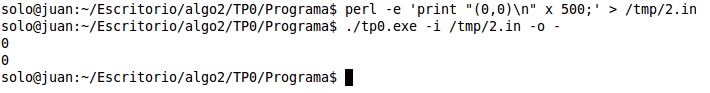
\includegraphics[width=1\textwidth]{prueba-2_con_problemas.png}
	\caption{Ejemplo 2 del enunciado del TP.}
	\label{fig:prueba2_con_prob}
\end{figure}

\begin{figure}[H]
	\centering
		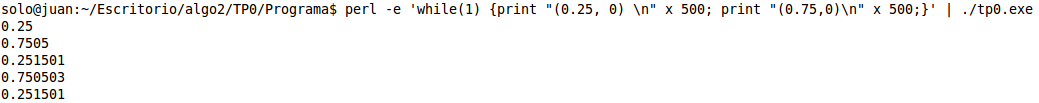
\includegraphics[width=1\textwidth]{prueba-3_con_problemas.png}
	\caption{Ejemplo 3 del enunciado del TP.}
	\label{fig:prueba3_con_prob}
\end{figure}

Como se puede ver en las Figuras \ref{fig:prueba1_con_prob} y \ref{fig:prueba2_con_prob}, el programa imprime un número por demás. Esto evidencia que al encontrarse con el final del archivo, vuelve a imprimir un complejo (algo que no debería suceder). Analizando el código se encontró el origen del error en el archivo \texttt{am\_proc.cc}

\begin{lstlisting}[firstnumber=100]
	if (is->eof())
		eof_flag=true;
\end{lstlisting}

A partir de este código se ve que al encontrar EOF cambia el valor de \texttt{eof\_flag} y continua con los demás comandos dentro del bucle, entre ellos la decimación e impresión. Si se insertan exactamente \texttt{N} complejos, ocurre una iteración indeseada. Para solucionar dicho problema se implementó lo siguiente

\begin{lstlisting}
	if(is->eof()){
		eof_flag=true;
		if(c==0)
			break;
	}
\end{lstlisting}

Se corrieron nuevamente las pruebas anteriores y a continuación se presentan los resultados

\begin{figure}[H]
	\centering
		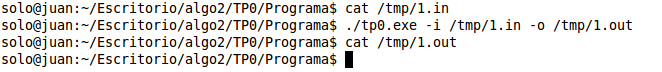
\includegraphics[width=1\textwidth]{prueba-1.png}
	\caption{Ejemplo 1 del enunciado del TP funcionando correctamente.}
	\label{fig:prueba1}
\end{figure}

\begin{figure}[H]
	\centering
		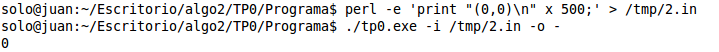
\includegraphics[width=1\textwidth]{prueba-2.png}
	\caption{Ejemplo 2 del enunciado del TP funcionando correctamente.}
	\label{fig:prueba2}
\end{figure}

Además, para probar si se obtiene el resultado correcto al insertar una cantidad que no sea múltiplo del número de decimación, se ejecutó el siguiente \emph{test}

\begin{figure}[H]
	\centering
		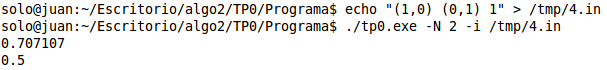
\includegraphics[width=1\textwidth]{prueba-5.png}
	\caption{Prueba al insertar una cantidad indivisible por el número de decimación}
	\label{fig_prueba5}
\end{figure}

Al mismo tiempo, se analizó el problema presentado en la Figura \ref{fig:prueba3_con_prob}. La causa de que los resultados tuvieran errores en los últimos 4 decimales fue la falta de inicialización de \texttt{c} al comenzar nuevamente el ciclo \texttt{while} del archivo \texttt{am\_proc.cc}. Ésto se solucionó de la siguiente manera:

\begin{lstlisting}
	for(i=1, c=0; i<=n_decimator && ((*is)>>aux); i++)
\end{lstlisting}

\begin{figure}[H]
	\centering
		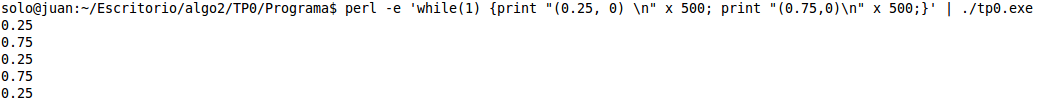
\includegraphics[width=1\textwidth]{prueba-3.png}
	\caption{Ejemplo 3 del enunciado del TP.}
	\label{fig:prueba3}
\end{figure}

Como se puede ver en la Figura \ref{fig:prueba3}, la implementación propuesta logró solucionar el problema previo. Cabe destacar que las capturas de pantalla expuestas, se realizaron al resolver ambos problemas en simultaneo. De lo contrario, la prueba de la Figura \ref{fig_prueba5} hubiera tenido el mismo error presentado por el problema original.

Por otro lado, se puso a prueba la interpretación de los números complejos. Se prueba si al ingresar una serie de coeficientes como la parte real, origina el mismo resultado que los mismos coeficientes pero como parte puramente imaginaria. En la siguiente Figura se exponen las corridas:

\begin{figure}[H]
	\centering
		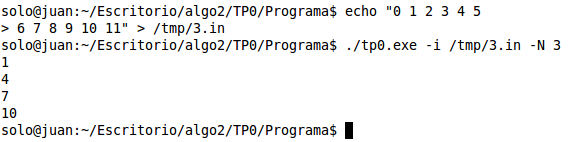
\includegraphics[width=1\textwidth]{prueba-4.png}
\end{figure}
\begin{figure}[H]
	\centering
		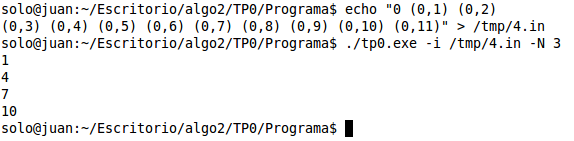
\includegraphics[width=1\textwidth]{prueba-4bis.png}
	\caption{Prueba con distintos números complejos}
	\label{fig:prueba-4}
\end{figure}

Finalmente se insertó una cadena de caracteres para ver cómo se comporta el programa ante un error en la entrada y el resultado, satisfactorio, se puede ver a continuación:

\begin{figure}[H]
	\centering
		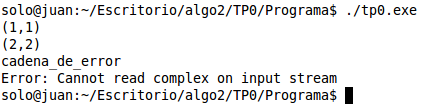
\includegraphics[width=1\textwidth]{prueba-6.png}
	\caption{Prueba ingresando no-complejos}
	\label{fig:prueba-6}
\end{figure}


	
	\section{Código fuente}
		

%	\lstlistoflistings
	\lstinputlisting{main.cc}
	\lstinputlisting{cmdline.h}
	\lstinputlisting{cmdline.cc}
	\lstinputlisting{complejo.h}
	\lstinputlisting{complejo.cc}
	\lstinputlisting{am_proc.h}
	\lstinputlisting{am_proc.cc}



\end{document}
